\ssn{3 March 2013}

\sssn{Pre-meeting discussion topics/ideas}

Following the discussion of bonuses from the previous meeting, Benjamyn wanted
to discuss his idea of bonus upgrade. The following is a list of ideas for
combining bonuses. However, bonus combination could be implemented after the
game has been more fully developed. Bonuses will have a limit on their
upgradability. By upgrading a bonus, this also opens up a bonus slot.
\benum
	\bolditem{bomb}{the radius of the bomb increases. The un-upgraded bomb has a
		single block radius and the radius increases by one block from every upgrade,
		reaching a maximum radius of 3 blocks.}
	\bolditem{slow down/speed up}{changes the rate by an extra 0.5x than if the
		speed was changed using each of these bonuses individually. Thus upgrading a
		slow down, will slow down the speed by 2.5x rather than 2x.}
	\bolditem{chain}{the lifetime of the chain increases}
	\bolditem{block}{the lifetime of the block increases}
\eenum

Benjamyn also wanted to discuss whether the block bonus can be used to complete
a layer.

\para{Double reward}
Currently, if a player completes a level, they are rewarded twice: once by
completing a level and reducing the distance that the blocks are to their
ceiling, and once for pushing the platform towards their opponent's ceiling.
Thus, after completing a level, their top most block actually moves a distance
of two units away from the ceiling.

Benjamyn had the following idea: depending on how many layers the player
completes, various rewards are given:
\bitem
	\bolditem{one layer}{all that occurs is that the layer disappears and the
		above blocks fall as in the original tetris}
	\bolditem{two layers}{the layer is removed and they receive a bonus}
	\bolditem{three layers}{the probability that the bonus they receive is more
		valuable increases}
	\bolditem{four (max) layers}{the platform changes location towards their
		opponent's ceiling and away from their ceiling}
\eitem

\para{Coding style/layout}

Benjamyn wanted to discuss the coding style/layout.

\para{Calendar}

We decided on 26 February in class that the main goal of the next meeting was
to develop a timeline for the project and to continue the previous meeting's
discussions.

\sssn{In-meeting discussion}

\para{Bonuses and Bonus upgrades}
Zach agreed with the idea and that the idea should be implemented if time
permitted. We additionally discussed the question of whether the block bonus
can be used in completing a layer. We decided that initially, the block bonus
will not have a lifetime, which in one aspect provides interesting gameplay in
that the player who uses the bonus on the other player's arena must be
extremely strategic about where the block is placed, since it could end up
helping the opponent. If there is time, we will add a timed block bonus. This
may even branch out into two separate bonuses with the behavior described here.

\figwpdf{meetings/pics}{superBlocks}{A set of superblocks to be included in the
T3D game. The axes of rotation are also included in the drawings.}{0.7}

\wrapfigpdf{meetings/pics}{block}{The fundamental block of which superblocks
are composed of. Blocks are drawn so that one of their corners is at the origin
and they lie in the positive quadrant.}{l}{0.3}{0.28}

\para{Completing layers}
Zach agreed with Benjamyn's idea and concurred that the previous level
completion scheme resulted in a player received a double bonus.

\para{Speed of blocks}
We discussed how the speed of the blocks falling towards the platform may
increase as the length of the game increases, asymptotically approaching a
maximum speed.

\para{Code style/layout}
After going through one of Zach's source files, Benjamyn and Zach found that
they have very similar coding styles and that a formal document describing code
style was not required. A MOU was made to document private methods and to place
doxygen comments in header files only. We also agreed that the \code{master}
branch should \emph{always} be in a buildable and playable state.

\para{Superblocks and Collision Queries}

A lengthy discussion pursued on the functionality and implementation of the
Superblock token. Figure \ref{fig:superBlocks} shows a series of superblocks
that we brainstormed up during the meeting and want to include in our game. The
figures show the axis of rotation for each of the superblocks.

\begin{figure}
	\centering
	\begin{subfigure}[b]{0.5\textwidth}
		\centering
		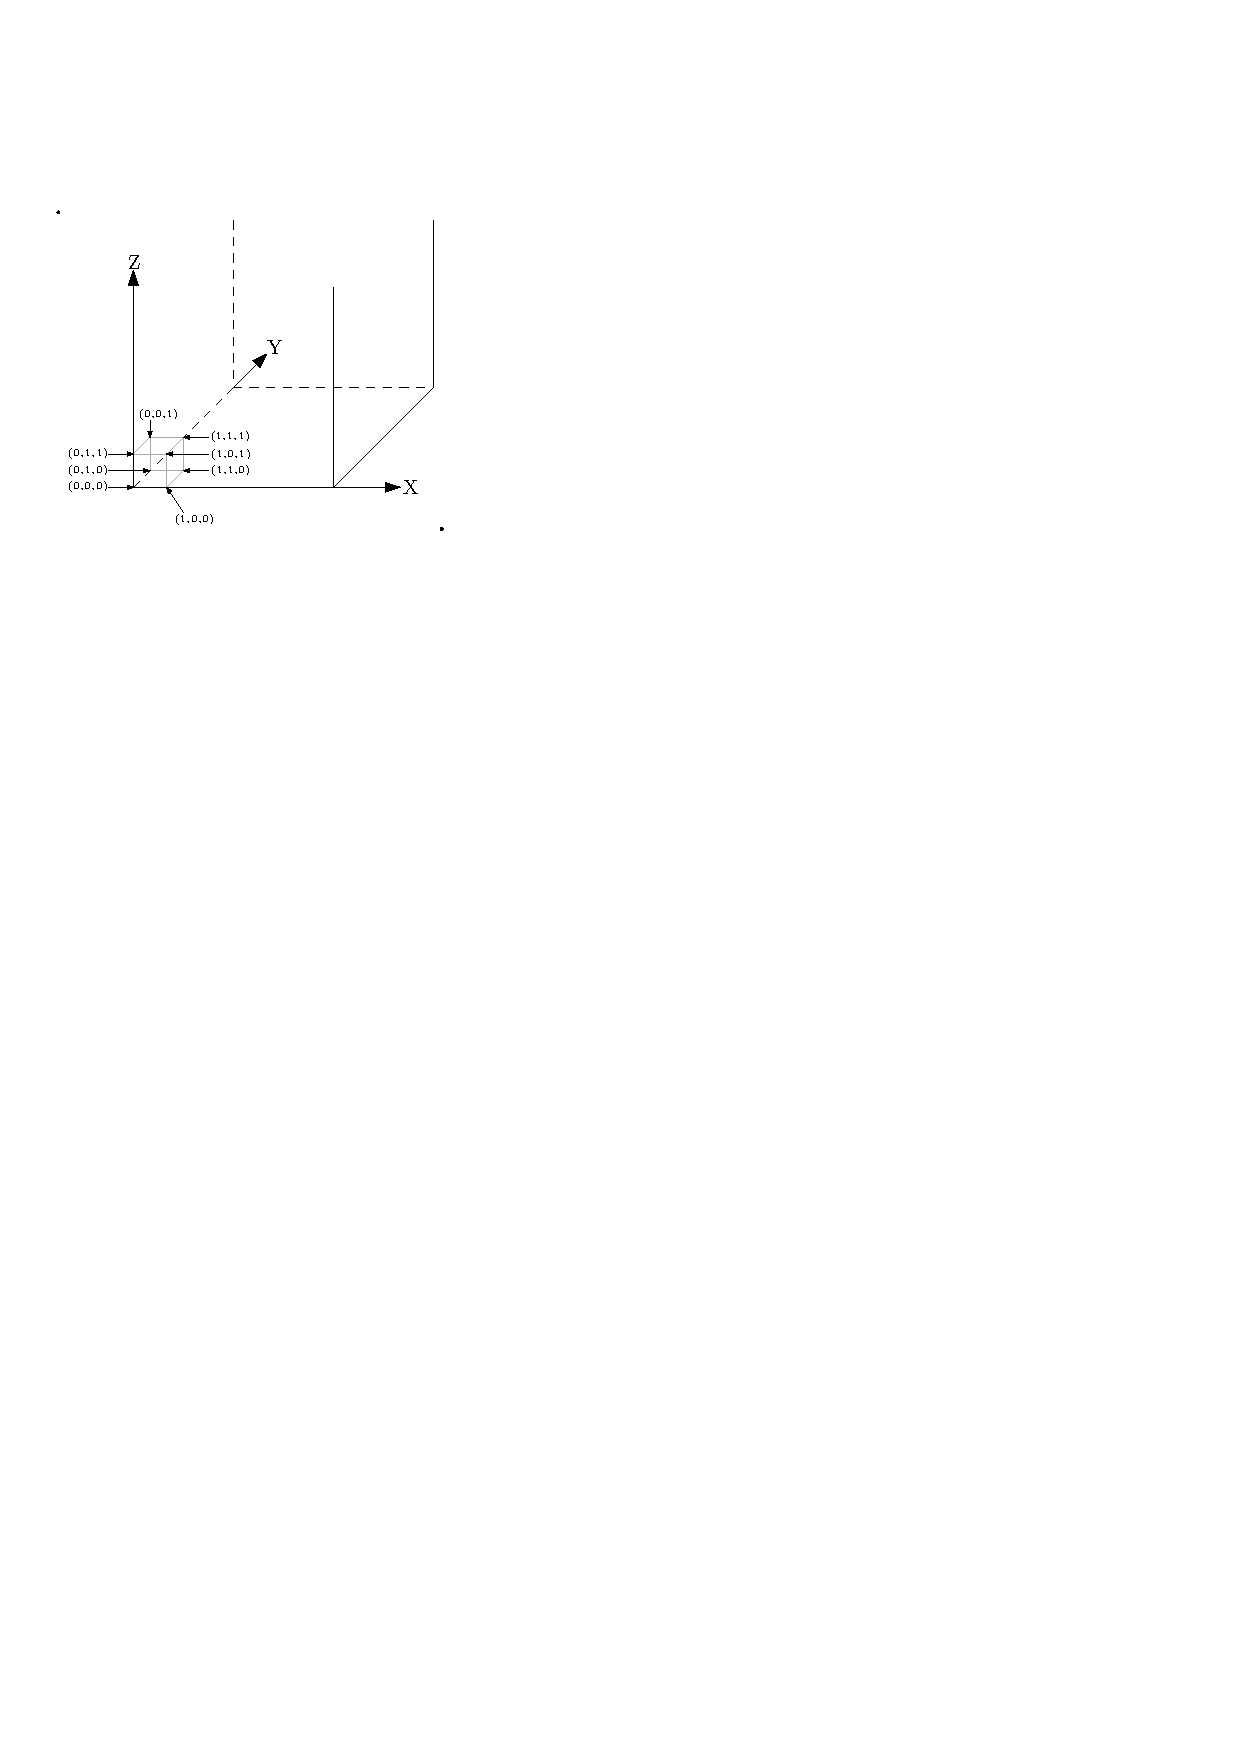
\includegraphics[width=1.0\textwidth]{meetings/pics/coords.pdf}
		\caption{Coordinates of the subarena.}
		\label{fig:coords}
	\end{subfigure}%
	\begin{subfigure}[b]{0.4\textwidth}
		\centering
		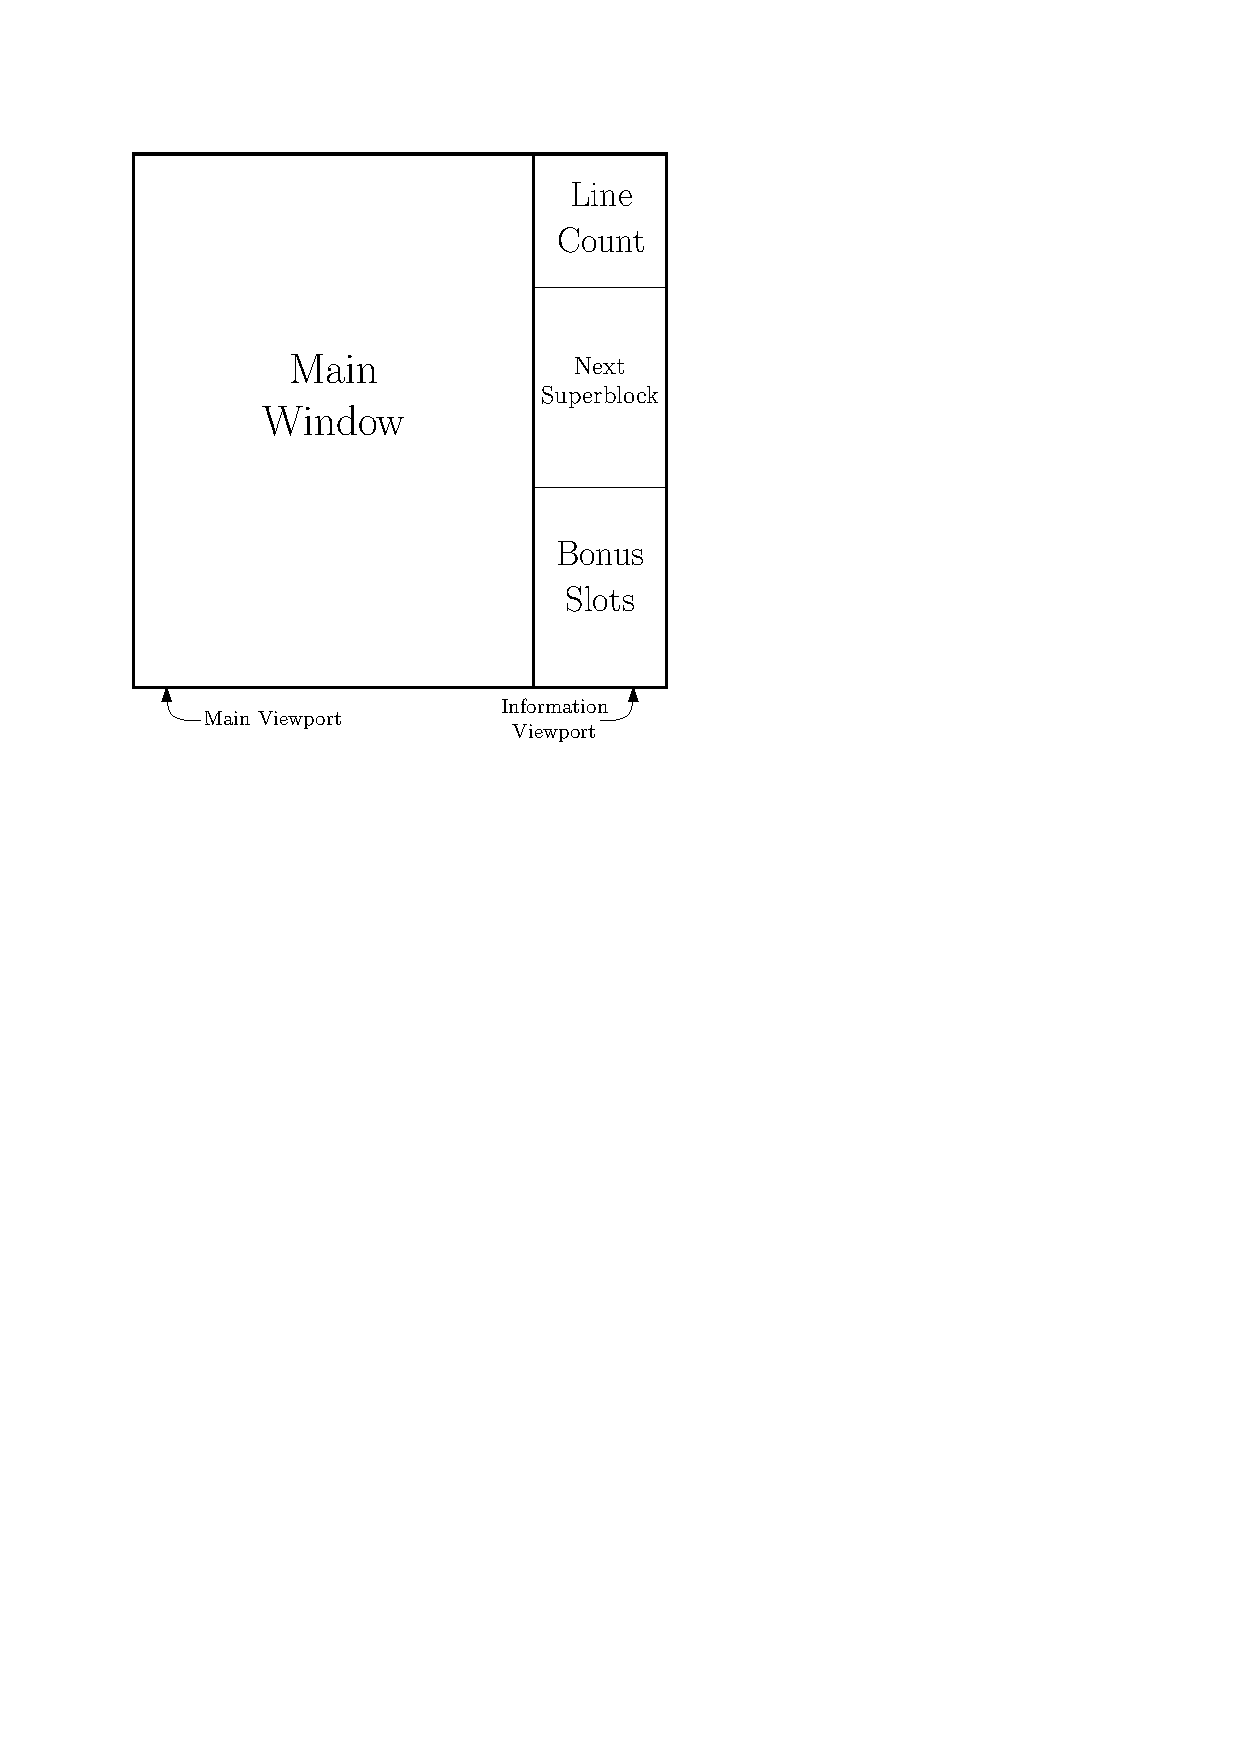
\includegraphics[width=0.9\textwidth]{meetings/pics/userInter.pdf}
		\caption{T3D user interface.}
		\label{fig:userInter}
	\end{subfigure}
\end{figure}

Each superblock is composed of basic blocks. Each block is a cube with sides of
length 1. The block is drawn so that the entire block is located in the
positive quadrant as show in figure \ref{fig:block}. In addition, one of the
block's corners is located at the origin. 

Individual blocks will possess no information about their orientation in space.
The superblocks will, however. The information contained in a superblock is the
set of blocks and their locations that compose the superblock, the rotation
point, and the rotations that have been applied to the superblock (caused by
the player).

The structure of the superblock plays itself into solving the problem of
collision queries. The superblock will be moving around in a subarena, either
due to the player applying rotations, the superblock naturally falling, or the
player causing the superblock to perform some sort of translation. Due to the
presence of other blocks in the subarena, the walls, and the platform, the move
requested must be validated.

The architecture was updated (figure \ref{fig:arch3Mar}) to include a token
that will handle collision queries. This token is best explained through
example. We may receive some keyboard input, such as a rotation to be applied
to the superblock. The command is forwarded to the superblock, which returns a
list of coordinates that the superblock will possess if the command were to be
committed. The collision query token then forwards these coordinates to the
subarea which will verify whether those positions are occuppied. If the
positions are unoccupied, then the collision query token will cause the command
to be applied.

The previous discussion led to how we want to represent the space of the
subarena. Since the blocks are defined by existing in the positive quadrant
with one of the corners to be the origin, we extended this definition to be
included for the subarena and layers as in figure \ref{fig:coords}. The
structure of the user interface and the substruct viewports is shown in figure
\ref{fig:userInter}.

\para{Calendar and Milestones}
We split the project up into three primary milestones, which are shown in table
\ref{tab:milestones}.

\begin{table}[!h]
	\centering
	\begin{tabular}{ | l | l | p{6cm} p{6cm} |}
		\hline
			& & & \\[1pt]
			\tb{Milestone} & \tb{Week} & \multicolumn{2}{c|}{\tb{Tasks}} \\[10pt]
		\hline
			\multirow{3}{*}{1} & 1 & world with camera & superblock production \\
			& 2 & ability to move superblock & spacebar: insert into layer \\
			& 3 & collision queries & \\
		\hline
			\multirow{2}{*}{2} & 4 & add player structure & user interface/viewport \\
			& 5 & layer completion & \\
		\hline
			\multirow{3}{*}{3} & 6 & two player interaction & bonuses \\
			& 7 & music & bonus upgrades \\
			& 8 & timer bonuses & \\
		\hline
			4 & 9 & game presentation & buildable and playable demo \\
		\hline
	\end{tabular}
	\caption{Schedule of tasks to get completed during each milestone time interval.}
	\label{tab:milestones}
\end{table}

\figw{meetings/pics}{calendar}{Calendar for game completion.}{1.0}



\figwpdf{meetings/pics}{arch3Mar}{An updated diagram of the soft architecture of the T3D
game.}{0.8}
